\documentclass[9pt,t,aspectratio=169]{beamer}
\usetheme[white]{Wisconsin}
\usepackage[utf8]{inputenc}
\setbeamertemplate{page number in head/foot}[totalframenumber]
\setbeamerfont{title}{size=\LARGE}
\setbeamerfont{subtitle}{size=\Large}
\setbeamerfont{block body}{size=\footnotesize}
\setbeamerfont{author}{size=\LARGE}
\setbeamerfont{date}{size=\Large}
\setbeamerfont{institute}{size=\large}
\setlength{\leftmargini}{0pt}


\usepackage{caption}
\captionsetup[figure]{labelformat=empty} % turn off labeling caption figures
%subcaptions
\usepackage{subcaption}
\captionsetup[subfigure]{labelformat=empty} % turn off labeling subcaption figures

% turn off Figure in captions
\usepackage{caption}
% \captionsetup[figure]{labelformat=empty}

\newcommand{\QOR}{\qquad \text{OR} \qquad}
\newcommand{\QAND}{\qquad \text{AND} \qquad}
\newcommand{\QTHUS}{\qquad \text{THUS} \qquad}
\newcommand{\QTHEN}{\qquad \text{THEN} \qquad}
\newcommand{\QWITH}{\qquad \text{WITH} \qquad}
\newcommand{\QFOR}{\qquad \text{FOR} \qquad}
\newcommand{\QSO}{\qquad \text{SO} \qquad}
\newcommand{\QWHERE}{\qquad \text{WHERE} \qquad}
\newcommand{\LINE}{\par\noindent\rule{\textwidth}{0.4pt}\par}
\newcommand{\toinf}{\rightarrow\infty}
\newcommand{\tozero}{\rightarrow0}
\newcommand{\qeq}{\overset{?}{=}}
\newcommand{\ceq}{\overset{\checkmark}{=}}
\renewcommand{\epsilon}{\varepsilon}
\newcommand{\keff}{$k_{e\!f\!f}$}
\newcommand{\kinf}{$k_{inf}$}

% table packages
\usepackage{booktabs}

% Roman Numerals
\newcommand{\rom}[1]{\expandafter\uppercase{\Romannumeral #1\relax}}

% hypersetup
\usepackage{hyperref}
\hypersetup{colorlinks,
            linkcolor = black,
            citecolor = black,
            urlcolor = cyan
}


\def\brac#1{\{#1\}}
\def\Brac#1{\big\{#1\big\}}
\def\BRAC#1{\bigg\{#1\bigg\}}
\def\angbrac#1{\langle#1\rangle}
\def\Angbrac#1{\big\langle#1\big\rangle}
\def\ANGBRAC#1{\bigg\langle#1\bigg\rangle}

% Transitional slides between sections
\AtBeginSection[]
{
    \begin{frame}
        \frametitle{Table of Contents}
        \tableofcontents[currentsection]
    \end{frame}
}


% Bibliography
\usepackage[sorting=none]{biblatex} %Imports biblatex package and cites in order of appearance
\addbibresource{physor2024_pres.bib} %Import the bibliography file
% make all font colors white
\setbeamercolor{bibliography item}{fg=black}
\setbeamercolor{bibliography entry author}{fg=black}
\setbeamercolor{bibliography entry title}{fg=black}
\setbeamercolor{bibliography entry location}{fg=black}
\setbeamercolor{bibliography entry note}{fg=black}
% adds numeric labels linked to bib entries
\setbeamertemplate{bibliography item}{\insertbiblabel}

% eliminate header within an environment
\makeatletter
    \newenvironment{withoutheadline}{
       \setbeamertemplate{headline}[default]
       \def\beamer@entrycode{\vspace*{-\headheight}}
    }{}
\makeatother

% appendix renumbering
\usepackage{appendixnumberbeamer}
% frame breaks with same title
\setbeamertemplate{frametitle continuation}[from second][]

\title{Exploring Effects of Homogenization on an OpenMC Depletion Analysis}
\subtitle{of a TRISO Fueled, Helium Cooled Microreactor}
\author{\vspace*{-0.45cm}Lewis I. Gross\textsuperscript{1}, Patrick Shriwise\textsuperscript{2,1}, Benjamin Lindley\textsuperscript{1} and Paul P.H. Wilson\textsuperscript{1}}
\institute{University of Wisconsin-Madison\textsuperscript{1}, Argonne National Lab\textsuperscript{2} }
\date{\vspace*{-0.25cm}April 24, 2024}
%%----------------------------------------------------------------------------%%
\begin{document}

\begin{withoutheadline}
\begin{frame}[plain] % the plain makes the first frame look good
    \maketitle
\end{frame}
\end{withoutheadline}

\author{Lewis Gross, Patrick Shriwise, Ben Lindley, and Paul Wilson} % reset author so affiliations don't show up in footer
%%----------------------------------------------------------------------------%%
%% Overview
%%----------------------------------------------------------------------------%%
\begin{withoutheadline}
\begin{frame}{Outline}
  \tableofcontents
\end{frame}
\end{withoutheadline}


%%----------------------------------------------------------------------------%%
%% Section 1
%%----------------------------------------------------------------------------%%
\section{Virtual Test Bed Gas-Cooled Microreactor}
\hypersetup{citecolor=white}
\begin{frame}{Virtual Test Bed \cite{vtb2023}}
    \begin{figure}
        \centering
        
\includegraphics[width=0.65\linewidth]{figures/nric_logo.png}
    \end{figure}
    \begin{figure}
        \centering
        
\includegraphics[width=0.6\linewidth]{figures/NEAMS.png}
    \end{figure}
\end{frame}


\begin{frame}{Microreactors \cite{INL_MR}}
    \begin{figure}
        \centering
        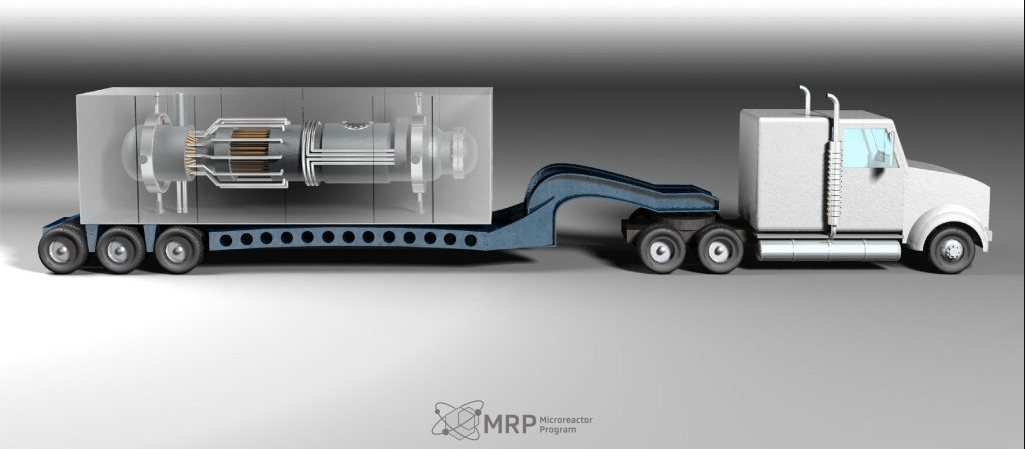
\includegraphics[width=0.95\linewidth]{figures/INL_MR.png}
    \end{figure}
\end{frame}
\hypersetup{citecolor=black}

\begin{frame}{TRISO Fuel}
    \begin{minipage}[t]{0.45\linewidth}
        \begin{figure}
            \centering
            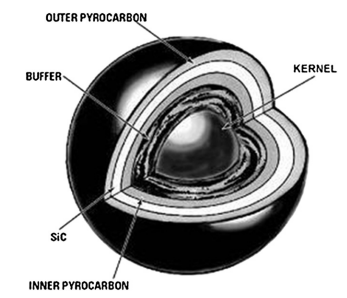
\includegraphics[width=0.9\linewidth]{figures/TRISO_diagram_Zhou_Tang.png}
            \caption{Layers from innermost to outermost: fuel kernel, buffer, Inner PyC, SiC,Outer PyC \cite{zhou_tang}.}
        \end{figure}
    \end{minipage}
    \hfill%
    \begin{minipage}[t]{0.45\linewidth}
        \begin{itemize}
            \item Common fuel for HTGRs
            \item UCO fuel kernel radius 212.5 microns
            \item Outer PyC radius 427.5 microns
            \item Melting temperature significantly higher than operational temperatures \cite{zhou_tang}
            \item Designed to contain fission products \cite{zhou_tang}
            \item Typically packed into graphite compacts or into spherical pebbles for PBRs
            \item TRISO modeling challenges
            \begin{itemize}
                \item Five surfaces per TRISO
                \item Many TRISOs per reactor
            \end{itemize}
        \end{itemize}
    \end{minipage}
\end{frame}

\begin{frame}{Virtual Test Bed Gas Cooled Microreactor (VTB GCMR)}
    \begin{minipage}[t]{0.525\linewidth}
        \begin{itemize}
            \item Existing VTB GCMR simulations
            \begin{itemize}
                \item Preliminary multiphysics models: Griffin-BISON-SAM \cite{Stauff-preliminary-applications-2021,Stauff-applications-2022,Abdelhameed-ANS-2022}
                \item Dynamic multiphysics simulations: flow blockage and Reactivity Insertion Accident \cite{HF_MRs_ANL}
                \item Balance of plant 1D thermal hydraulic simulation \cite{Duchnowski_plant_balance_2022}
            \end{itemize}
            \item This work presents the first published OpenMC Model of the VTB GCMR
            \begin{itemize}
                \item Plans to add this work's model to the VTB this summer
            \end{itemize}
            \item For a full core model, it will be prohibitively expensive to model every TRISO explicitly
        \end{itemize}
    \end{minipage}
    \hfill%
    \begin{minipage}[t]{0.425\linewidth}
        \begin{figure}
            \centering
            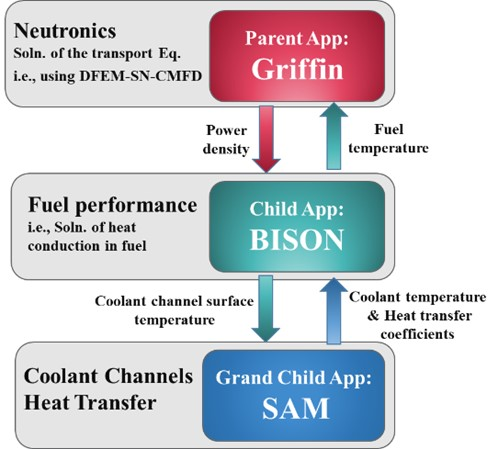
\includegraphics[width=0.875\linewidth]{figures/gcmr_preliminary_mutliapps.png}
            \caption{MultiApp hierarchy of preliminary GCMR models. Image from \cite{Abdelhameed-ANS-2022}.}
        \end{figure}
    \end{minipage}

\end{frame}

\begin{frame}{Research Goal}
    \begin{itemize}
        \item \textbf{What degree of explicitness is required to represent TRISO for a full-core GCMR model?}
        \item To answer this question, varying degrees of homogenization were used in an infinite-assembly depletion model, computing \kinf~as a function of burnup up to 29 GWd/tonne-U.
        \item Since this reactor is intended for load-following, a burnup simulation was conducted at 100\%, 50\%, and 10\% of full power (225 KWt).
        \item Two homogenization strategies: ``\textbf{kernel only}'' and ``\textbf{full volume}''
        \item Kernel only homogenizes all non-fuel TRISO layers by volume fraction into the background graphite.
        \item It then packs UCO kernels with the same original positions as in the fully explicit case.
        \item Full volume homogenizes all material within a compact by their volume fraction into a single material.
        \item Comparing both homogenizations to the fully explicit case can be used as a basis for deciding how proceed with a full core model.
    \end{itemize}
\end{frame}

%%----------------------------------------------------------------------------%%
%% Section 2
%%----------------------------------------------------------------------------%%
\section{OpenMC Model}

\begin{frame}{OpenMC Model}
    \begin{minipage}[t]{0.2\linewidth}
        \begin{figure}
            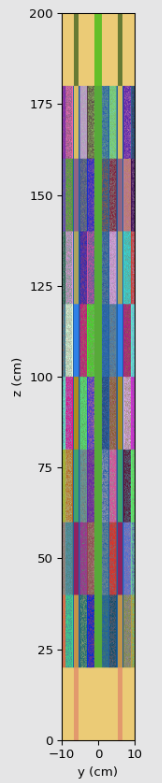
\includegraphics[height=0.7\textheight]{figures/yz_slice.png}
            \caption{YZ slice of reactor}
        \end{figure}
    \end{minipage}
    \begin{minipage}[t]{0.365\linewidth}
        \begin{figure}
            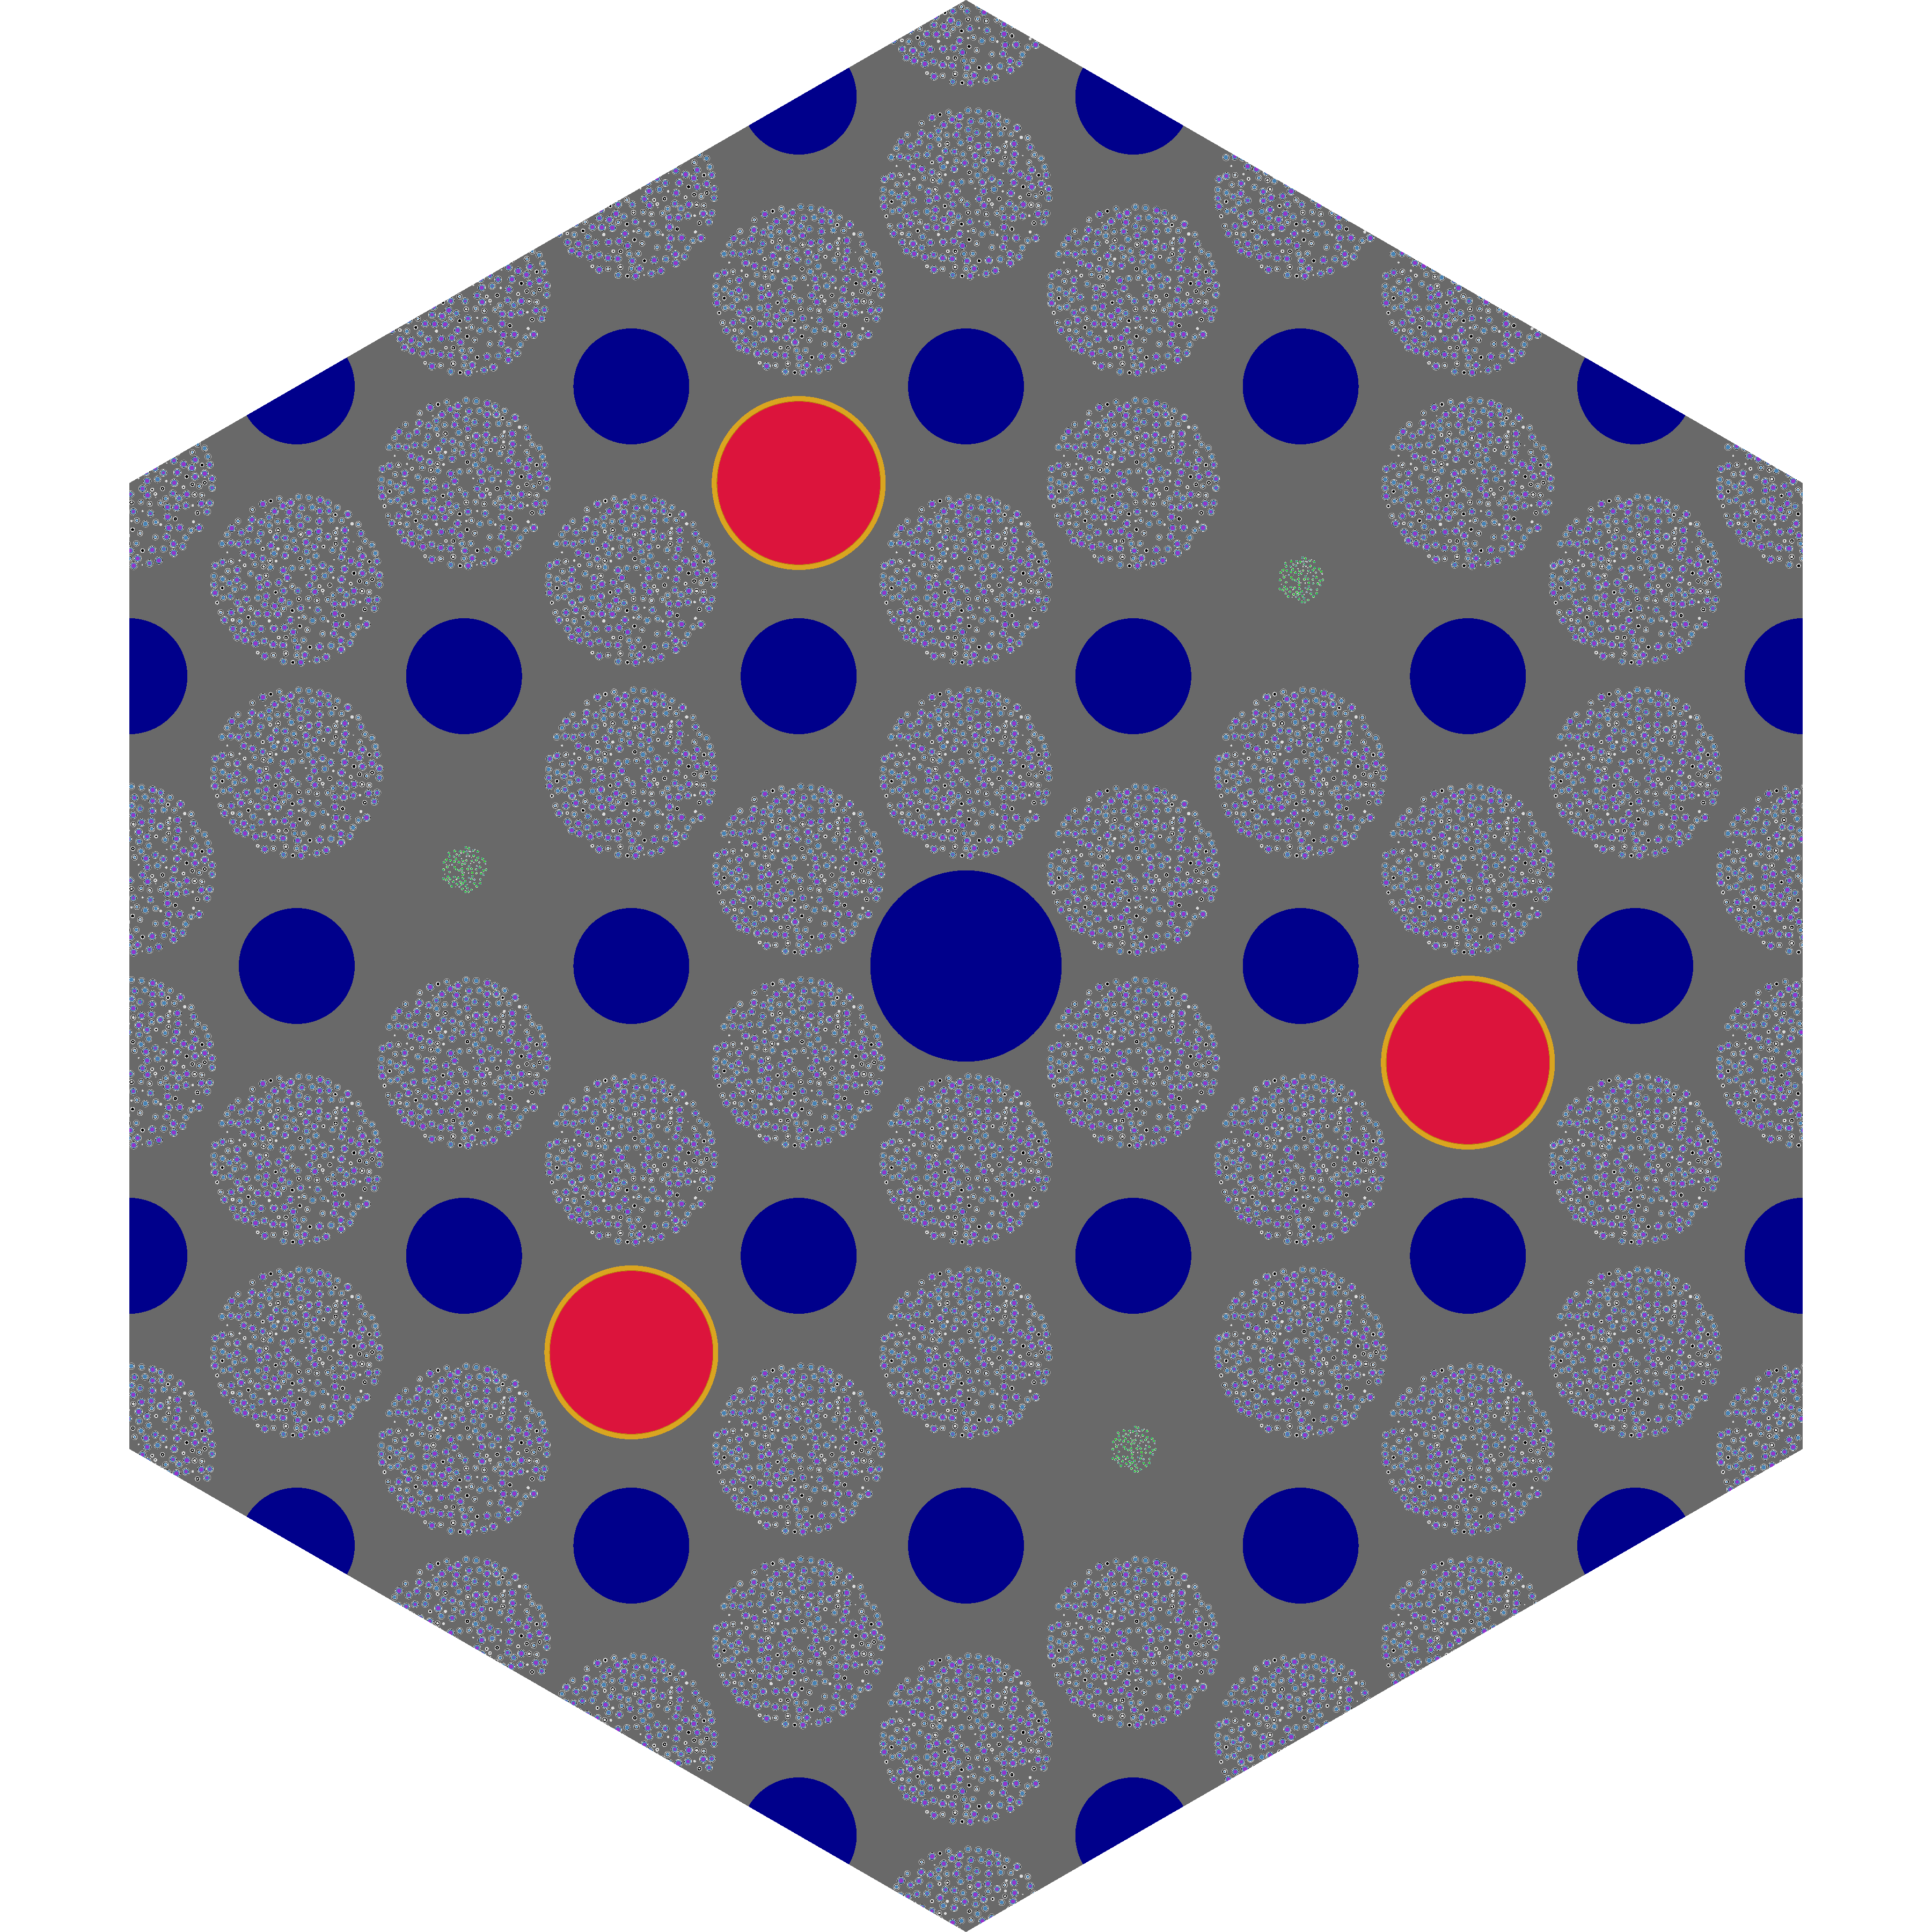
\includegraphics[height=0.7\textheight]{figures/gcmr_slice.png}
            \caption{XY slice of reactor}
        \end{figure}
    \end{minipage}
    \hfill%
    \begin{minipage}[t]{0.385\linewidth}
        \begin{itemize}
        \item materials in XY slice
        \begin{itemize}
            \item gray = graphite
            \item blue = helium
            \item red = YH2 moderator
            \item gold = FeCrAL envelope
            \item green = B4C poison spheres
            \item purple dots = TRISO
        \end{itemize}
        \item 8 axial layers in the core
        \item 2 axial layers per reflector
        \item pin pitch = 2cm
        \item periodic BC on hexagonal boundary
        \item vacuum BC at z = 0, z = 200 cm
        \item 3-way symmetry cloning scheme
        \item images via openmc-plotter
        \end{itemize}
    \end{minipage}
\end{frame}

\begin{frame}{System Parameters}
    \begin{table}[h]
        \centering
        \begin{tabular}{|c|c|c|}
            \hline
            \multicolumn{3}{|c|}{\textbf{geometric parameters}} \\
            \hline
            fuel compact radius & poison compact radius & moderator compact radius  \\
            0.90 cm & 0.25 cm   & 0.843 cm  \\
            \hline
            control compact radius & coolant compact radius & FeCrAl thickness \\
            0.99 cm    & 0.60 cm & 0.05 cm \\
            \hline
            Cr coating thickness & reflector heights & core height \\
            \hline
            0.007 cm & 20 cm & 160 cm \\
            \hline
        \multicolumn{3}{c}{} \\
        \multicolumn{3}{c}{} \\
        \hline
        \multicolumn{3}{|c|}{\textbf{operation and design parameters}} \\
        \hline
        fuel packing fraction & poison packing fraction  & enrichment \\
        \hline
        0.4 -  & 0.25 - &  19.95\% \\
        \hline
        inlet temperature & outlet temperature & outlet pressure \\
        \hline
        873.15 K & 1133.65 K  & 7 MPa \\
        \hline
        \end{tabular}
        \label{tab:operational_params}
    \end{table}
\end{frame}

\begin{frame}{Depletion Theory}
    \begin{itemize}
        \item Depletion simulations numerically solve the Bateman equations for the number densities $N_{i}(t)$:
        \begin{multline} \label{eq:batemen}
            \frac{dN_{i}}{dt} =
            \sum_{j} \bigg[\int_{0}^{\infty} \sigma_{j\rightarrow{i}}(E,t)\phi(E,t)dE + \lambda_{j\rightarrow{i}}\bigg]N_{j}(t) \\
            -\bigg[\int_{0}^{\infty} \sigma_{i}(E,t)\phi(E,t)dE
            +\sum_{j}\lambda_{i\rightarrow{j}}\bigg] N_{i}(t).
        \end{multline}
        \begin{itemize}
            \item $\sigma_{j\rightarrow{i}}(E,t)$ = transmutation cross section of isotope $j$ that produces isotope $i$ at energy $E$ at time $t$
            \item $\phi(E,t)$ = energy and time dependent flux
            \item $\lambda_{j\rightarrow{i}}$ = decay constants for decay modes in nuclide $j$ that produce nuclide $i$
        \end{itemize}
        \item We can represent the system of equations in matrix form to solve for a nuclide vector $\textbf{N}(t)\in\mathbb{R}^{n}$
        \begin{equation} \label{eq:burnup matrix odes}
            \frac{d\textbf{N}}{dt} =
            \textbf{A}(\textbf{N},t) \textbf{N}
            \QWITH
            \textbf{N}(0) = \textbf{N}_{0},
        \end{equation}
        where $\textbf{A}\in\mathbb{R}^{n\times n}$ is commonly referred to as the burnup matrix.
    \end{itemize}
\end{frame}

\begin{frame}{Depletion Theory}
    \begin{itemize}
        \item Assuming $\textbf{A}(\textbf{N},t)$ changes slowly enough over time that it can be approximated as constant within a timestep (quasi steady-state assumption) gives
        \begin{equation} \label{eq:separable burnup matrix odes}
            \frac{d\textbf{N}}{dt} =
            \textbf{A} \textbf{N}
            \QWITH
            \textbf{N}(0) = \textbf{N}_{0}.
        \end{equation}
        \item The solution to which is
        \begin{equation} \label{eq:separation solution}
            \textbf{N}(t) = e^{\textbf{A}t} \textbf{N}_{0}.
        \end{equation}
        \item Since \textbf{A} technically does change in time (via $\textbf{N}(t)$ changing), it needs to be updated accordingly.
        \vspace*{0.4cm}
        \item Solving (\ref{eq:separable burnup matrix odes}) numerically involves two components \cite{romano-depletion-2021}:
        \begin{enumerate}
            \item Using a numerical method to integrate the matrix $\textbf{A}$ in (\ref{eq:separable burnup matrix odes}) forward in time. This usually involves taking one or more matrix exponential.
            \item Evaluating the matrix exponential $\exp(\textbf{A}t)$ or the action of the matrix exponential on a vector of nuclide concentrations.
        \end{enumerate}
    \end{itemize}
\end{frame}

\begin{frame}{OpenMC Depletion Settings}
    \begin{itemize}
        \item Predictor-Corrector time integration scheme
        \begin{itemize}
            \item requires two transport solves per time step
            \item Constant Extrapolation/Constant Midpoint scheme from Isotalo et al. \cite{isotalo_comparison_2015}
            \item $k$-eigenvalue simulations used 25 inactive and 75 active batches with 10000 particles per batch
            \item continuous energy cross sections from ENDF-B-VII.1
        \end{itemize}
        \item Chain XML file
        \begin{itemize}
            \item contains transmutation and decay data necessary to compute the burnup matrix
            \item based on the CASL project \cite{CASL-report}, which uses a thermal spectrum to compute the burnup matrix
            \item provided by OpenMC \cite{openmc-chains}
        \end{itemize}
        \item Time Steps - kept total burnup the same at each step in the simulation
        \begin{itemize}
            \item Full power time steps: \texttt{[1]*5 + [5]*3 + [15]*3 + [60]*17} (days)
            \item Half power time steps: \texttt{[2]*5 + [10]*3 + [30]*3 + [120]*17} (days)
            \item Tenth power time steps: \texttt{[10]*5 + [50]*3 + [150]*3 + [600]*17} (days)
        \end{itemize}
    \end{itemize}
\end{frame}
%%----------------------------------------------------------------------------%%
%% Section 3
%%----------------------------------------------------------------------------%%
\section{Results and Discussion}

\begin{frame}{Fully-explicit \kinf~versus burnup with $2\sigma$ error bars up to $\sim$29 GWd/tonne-U}
    \begin{figure}
        \vspace*{-0.4cm}
        \centering
            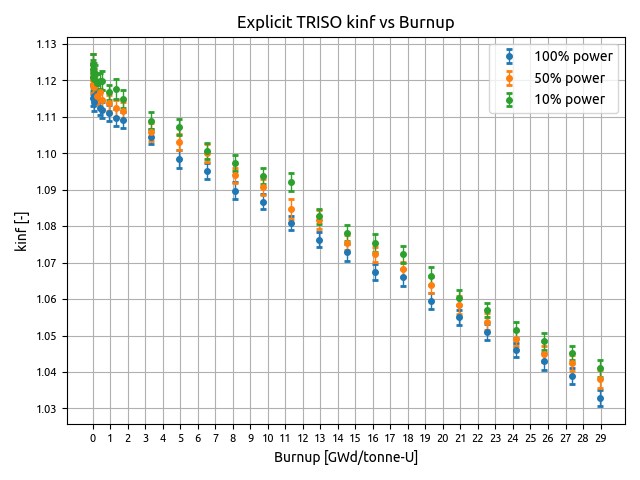
\includegraphics[height=0.9\textheight]{figures/expl_kinf_vs_bu.png}
        \label{fig:kinf_full_explicit_results}
    \end{figure}
\end{frame}

\begin{frame}{Comparing Eigenvalues}
    \Large
    \begin{itemize}
        \item Denote the first set of eigenvalues $k_ 1$ and the second set $k_2$, the $\Delta \rho$ between them is given by
        \begin{equation}
            \Delta \rho \equiv
            \rho_1 - \rho_2 =
            \frac{k_1-1}{k_1} - \frac{k_2 - 1 }{k_2} =
            \frac{1}{k_2} - \frac{1}{k_1}
        \end{equation}
        \item Average $\Delta \rho$ compared with the explicit reference at every power with $2\sigma$ uncertainties
        \begin{table}[!h]
            \centering
            \begin{tabular}{c|c|c}
            $\overline{\Delta \rho}$ & explicit - homogenized & explicit - kernel only \\ \hline
            100\% power & 1533 $\pm$ 55 pcm &  -158 $\pm$ 55 pcm \\
            50\% power & 1495 $\pm$ 56 pcm & -193 $\pm$ 55 pcm\\
            10\% power & 1529 $\pm$ 56 pcm  & -203 $\pm$ 55 pcm
            \end{tabular}
            \label{tab:average_pcms}
        \end{table}
    \item Kernel only $\Delta \rho$ on average performs about 1 order of magnitude better than full homogenization.
    \end{itemize}
    \normalsize
\end{frame}

\begin{frame}{$\Delta \rho$ with $2\sigma$ error as a function of burnup  up to $\sim$29 GWd/tonne-U}
    \begin{figure}
        \centering
        \begin{subfigure}{0.495\linewidth}
            \centering
            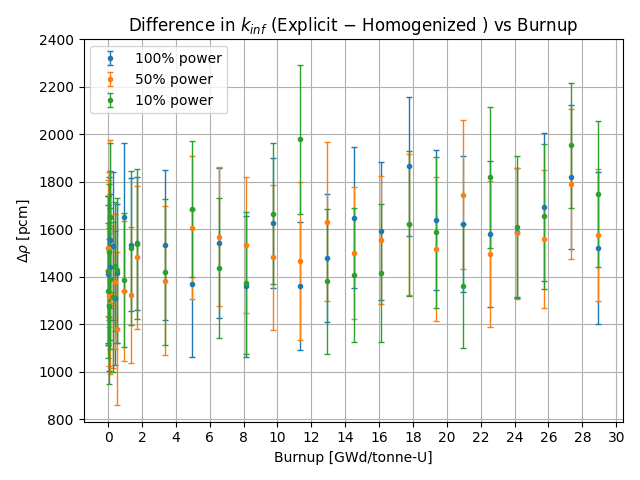
\includegraphics[width=\linewidth]{figures/explicit_minus_homog.png}
        \end{subfigure}
        \begin{subfigure}{0.495\linewidth}
            \centering
            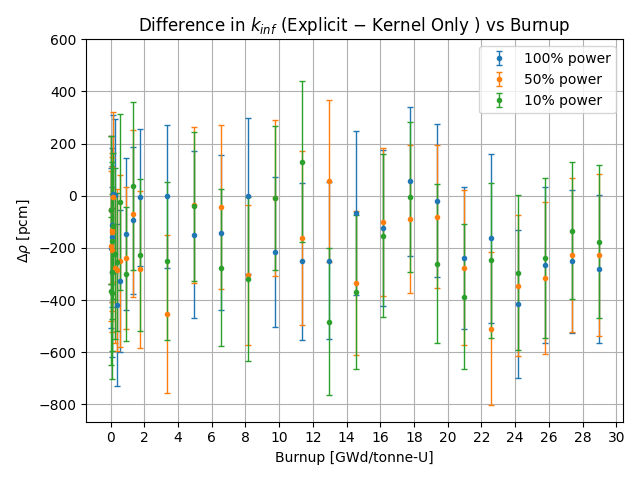
\includegraphics[width=\linewidth]{figures/explicit_minus_kern.png}
        \end{subfigure}
        \label{fig:pcm_diffs}
    \end{figure}
\end{frame}


%%----------------------------------------------------------------------------%%
%% Section 4
%%----------------------------------------------------------------------------%%
\section{Next Steps}
\begin{frame}{Two-layer TRISO Homogenization}
    \begin{itemize}
        \item While the kernel only eigenvalue computation outperforms the fully homogenized in terms of accuracy, it would be desirable to lower $\Delta \rho$ below 100 pcm.
        \item One potential source of error in the kernel only model is the effect of moving SiC.
        \item The kernel only model moves SiC further from the fuel than it exists in the explicit model.
        \begin{itemize}
            \item Typically, SiC is located in a spherical region 175 - 215 microns away from fuel.
        \end{itemize}
        \item Si has a much higher $\alpha = (\frac{A-1}{A+1})^2$ than C, so moving it away from fuel and replacing it with more graphite than in the explicit case increases the thermalization of neutrons near the fuel.
        \begin{itemize}
            \item Accordingly, more neutrons will escape the resonance region than should.
            \item This explains why $\Delta \rho$ is negative for explicit minus kernel
        \end{itemize}
        \item A next iteration on fuel homogenization would be to leave the graphite background alone and only homogenize within a TRISO to create a \textbf{two layer} homogenization that packs TRISO fuel particles with a UCO fuel kernel at the center and all other layers homogenized together. 
    \end{itemize}
\end{frame}

%%----------------------------------------------------------------------------%%`'
%% Bibliography
%%----------------------------------------------------------------------------%%

\begin{withoutheadline}
    \begin{frame}{Acknowledgements}
        \begin{itemize}
            \item The first author was supported in part by the US Nuclear Regulatory Commission's Graduate Fellowship Program administered by the University of Wisconsin-Madison.
            \item The OpenMC team!
            \item The Center for High Throughput Computing at the University of Wisconsin - Madison
            \item Co-authors: Patrick Shriwise, Benjamin Lindley, and Paul P.H.~Wilson.
        \end{itemize}
        \begin{figure}[H]
            \centering
            
\includegraphics[height=0.3\textheight]{figures/openmc_logo.png}
        \end{figure}
        \begin{figure}[H]
            \centering
            
\includegraphics[height=0.3\textheight]{figures/CHTC.png}
        \end{figure}
    \end{frame}
\end{withoutheadline}

\begin{withoutheadline}
    \begin{frame}[allowframebreaks]{Bibliography}
        \printbibliography
    \end{frame}
\end{withoutheadline}

\begin{withoutheadline}
    \LARGE
    \begin{frame}{Open Source Projects}
        \begin{itemize}
            \item OpenMC website: \href{https://openmc.org/}{https://openmc.org/}
            \item OpenMC repository: \href{https://github.com/openmc-dev/openmc}{https://github.com/openmc-dev/openmc}
            \item VTB: \href{https://mooseframework.inl.gov/virtual_test_bed/}{https://mooseframework.inl.gov/virtual\_test\_bed/}
            \item VTB repository: \href{https://github.com/idaholab/virtual_test_bed}{https://github.com/idaholab/virtual\_test\_bed}
            \item Add me on LinkedIn (\href{https://www.linkedin.com/in/lewisgross1296}{lewisgross1296}) and GitHub (\href{https://github.com/lewisgross1296}{lewisgross1296})!
        \end{itemize}
    \end{frame}
\end{withoutheadline}

\appendix

\begin{frame}{Equilibrium Xenon-135 Number Densities}
    \LARGE
    \begin{table}
        \centering
        \caption{All units are atom per cubic centimeter. Since the first five time steps are used to converge xenon, the numbers below are the average of the fifth to the last value for xenon number density.}
        \begin{tabular}{|c|c|c|c|} \hline
        representation & explicit & kernel only & homogenized \\ \hline
        100\% power & $2.43127\times 10^{16}$ & $2.41845\times 10^{16}$ & $1.19125\times 10^{15}$ \\  \hline
        50\% power & $1.31047\times 10^{16}$ & $1.30864\times 10^{16}$ & $6.45668\times 10^{14}$ \\ \hline
        10\% power & $2.82398\times 10^{15}$ & $2.81919\times 10^{15}$ & $1.38810\times 10^{14}$ \\ \hline
        \end{tabular}
        \label{tab:xenons}
    \end{table}
    \begin{itemize}
        \item These equilibrium values explain the observed trend at fresh fuel -- and for much of the simulation -- that lower power with the same total burnup has more excess Reactivity.
        \item The higher the power, the more Xenon-135 is produced during the initial jump to steady state, contributing to a larger negative reactivity insertion.
    \end{itemize}
\end{frame}

\begin{frame}{Plutonium 241 at Each Power for the Fully Explicit Case}
    \begin{figure}
        \vspace*{-0.4cm}
        \centering
            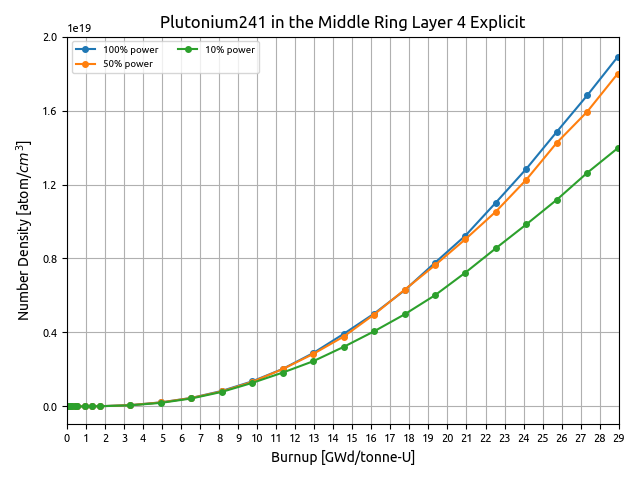
\includegraphics[height=0.9\textheight]{figures/explicit_Pu_241.png}
    \end{figure}
\end{frame}

\end{document}
